\documentclass{article}
\usepackage[utf8]{inputenc}
\usepackage{amsmath}
\usepackage{graphicx}
\usepackage{listings}
\usepackage{geometry}
\geometry{a4paper, margin=1in}
\usepackage{tikz}
\usetikzlibrary{trees}

\title{New York University \\ Tandon School of Engineering \\ Department of Computer Science and Engineering \\ Introduction to Operating Systems \\ Fall 2024 \\ Assignment 4 (10 points)}
\author{}
\date{}

\begin{document}

\maketitle

\section*{Problem 1 (2 points)}

If you create a main() routine that calls fork() twice, i.e., if it includes the following code:

\texttt{pid\_t x=-11, y=-22;}\\
\texttt{x = fork();}\\
\texttt{if(x==0) y = fork();}\\

Assuming all fork() calls succeed, draw a process tree similar to that of Fig. 3.8 (page 116) in your textbook, clearly indicating the values of x and y for each process in the tree (i.e., whether 0, -11, -22, or larger than 0). Note that the process tree should only have one node for each process and thus the number of nodes should be equal to the number of processes. The process tree should be a snapshot just after all forks completed but before any process exists. Each line/arrow in the process tree diagram shall represent a creation of a process, or alternatively a parent/child relationship.

\begin{center}
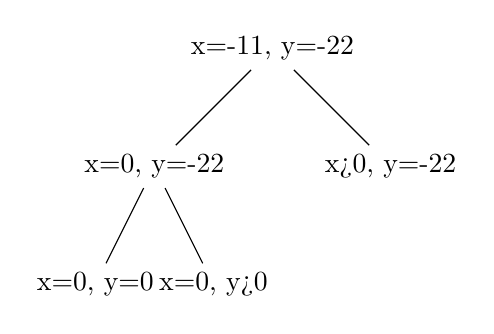
\begin{tikzpicture}[level distance=1.5cm,
  level 1/.style={sibling distance=3cm},
  level 2/.style={sibling distance=1.5cm}]
  \node (A) {x=-11, y=-22}
    child {node (B) {x=0, y=-22}
      child {node (D) {x=0, y=0}}
      child {node (E) {x=0, y>0}}
    }
    child {node (C) {x>0, y=-22}};
\end{tikzpicture}
\end{center}


\section*{Problem 2 (4 points)}

Write a program that creates the process tree shown below:

\begin{center}
\begin{tikzpicture}[level distance=1.5cm,
  level 1/.style={sibling distance=3cm},
  level 2/.style={sibling distance=1.5cm}]
  \node (A) {P1}
    child {node (B) {P2}
      child {node (D) {P4}}
      child {node (E) {P5}}
    }
    child {node (C) {P3}};
\end{tikzpicture}
\end{center}

\begin{lstlisting}[language=C, caption=Process Tree Creation]
#include <stdio.h>
#include <stdlib.h>
#include <unistd.h>
#include <sys/wait.h>

int main() {
    pid_t pid1, pid2, pid3, pid4, pid5;

    pid1 = getpid();
    printf("Process P1 (PID: %d) started.\n", pid1);

    pid2 = fork();
    if (pid2 < 0) {
        perror("fork failed");
        exit(1);
    } else if (pid2 == 0) {
        printf("Process P2 (PID: %d) started.\n", getpid());

        pid4 = fork();
        if (pid4 < 0) {
            perror("fork failed");
            exit(1);
        } else if (pid4 == 0) {
            printf("Process P4 (PID: %d) started.\n", getpid());
            exit(0);
        } else {
            pid5 = fork();
            if (pid5 < 0) {
                perror("fork failed");
                exit(1);
            } else if (pid5 == 0) {
                printf("Process P5 (PID: %d) started.\n", getpid());
                exit(0);
            } else {
                wait(NULL);
                wait(NULL);
                printf("Process P2 (PID: %d) finished.\n", getpid());
                exit(0);
            }
        }
    } else {
        pid3 = fork();
        if (pid3 < 0) {
            perror("fork failed");
            exit(1);
        } else if (pid3 == 0) {
            printf("Process P3 (PID: %d) started.\n", getpid());
            exit(0);
        } else {
            wait(NULL);
            wait(NULL);
            wait(NULL);
            printf("Process P1 (PID: %d) finished.\n", pid1);
            exit(0);
        }
    }
    return 0;
}
\end{lstlisting}


\section*{Problem 3 (4 points)}

Write a program whose main routine obtains a parameter n from the user (i.e., passed to your program when it was invoked from the shell, n>2) and creates a child process. The child process shall then calculate and print the sum of the first n even numbers. The parent waits for the child to exit and then prints the sum of the first n odd numbers. Do not use IPC in your solution to this problem (i.e., neither shared memory nor message passing).

\begin{lstlisting}[language=C, caption=Even and Odd Sum Calculation]
#include <stdio.h>
#include <stdlib.h>
#include <unistd.h>
#include <sys/wait.h>
#include <errno.h>

int main(int argc, char *argv[]) {
    if (argc != 2) {
        fprintf(stderr, "Usage: %s <n>\n", argv[0]);
        return 1;
    }

    long long n = atoll(argv[1]);
    if (n <= 2) {
        fprintf(stderr, "n must be greater than 2\n");
        return 1;
    }

    pid_t pid = fork();
    if (pid < 0) {
        perror("fork failed");
        return 1;
    } else if (pid == 0) { // Child process
        long long sum_even = 0;
        for (long long i = 1; i <= n; i++) {
            sum_even += 2 * i;
        }
        printf("Child: Sum of first %lld even numbers: %lld\n", n, sum_even);
        exit(0);
    } else { // Parent process
        wait(NULL);
        long long sum_odd = 0;
        for (long long i = 1; i <= n; i++) {
            sum_odd += (2 * i - 1);
        }
        printf("Parent: Sum of first %lld odd numbers: %lld\n", n, sum_odd);
        exit(0);
    }
    return 0;
}
\end{lstlisting}


\section*{Problem 4 (2 points)}

Explain the difference between a process and a thread.  Give examples of when you might prefer to use threads over processes, and vice-versa.

Processes are independent, self-contained execution environments, each with its own memory space, resources, and process ID. Threads, on the other hand, are lightweight units of execution within a process.  They share the same memory space and resources as other threads within the same process.

Threads are preferred when you need concurrency within a single task, minimizing the overhead of creating and managing separate processes.  Examples include handling multiple network connections in a server or performing parallel computations on a shared data set.  Processes are preferred when isolation and protection are paramount, as they prevent one process from corrupting another's memory space. Examples include running untrusted code or managing independent tasks that require strong isolation.


\section*{Problem 5 (4 points)}

Write a C program that uses pthreads to compute the factorial of a number entered by the user.  The program should create a separate thread to compute the factorial and then print the result in the main thread.  Ensure proper synchronization between the threads.


\begin{lstlisting}[language=C, caption=Pthread Factorial Calculation]
#include <stdio.h>
#include <stdlib.h>
#include <pthread.h>

long long factorial = 1;
long long num;
pthread_mutex_t mutex;

void* compute_factorial(void* arg) {
    long long n = *(long long*)arg;
    for (long long i = 1; i <= n; i++) {
        pthread_mutex_lock(&mutex);
        factorial *= i;
        pthread_mutex_unlock(&mutex);
    }
    pthread_exit(NULL);
}

int main() {
    pthread_t tid;
    pthread_mutex_init(&mutex, NULL);

    printf("Enter a number: ");
    scanf("%lld", &num);

    pthread_create(&tid, NULL, compute_factorial, &num);
    pthread_join(tid, NULL);

    printf("Factorial of %lld = %lld\n", num, factorial);
    pthread_mutex_destroy(&mutex);
    return 0;
}

\end{lstlisting}


\section*{Problem 6 (2 points)}

Describe the concept of a race condition and provide an example in a simple C program that uses multiple threads.  Explain how to prevent it.


A race condition occurs when multiple threads access and manipulate shared data concurrently, and the final outcome depends on the unpredictable order in which the threads execute. This leads to non-deterministic and often incorrect results.

\begin{lstlisting}[language=C, caption=Race Condition Example]
#include <stdio.h>
#include <pthread.h>

int counter = 0;

void* increment_counter(void* arg) {
    for (int i = 0; i < 1000000; i++) {
        counter++;
    }
    return NULL;
}

int main() {
    pthread_t tid1, tid2;

    pthread_create(&tid1, NULL, increment_counter, NULL);
    pthread_create(&tid2, NULL, increment_counter, NULL);

    pthread_join(tid1, NULL);
    pthread_join(tid2, NULL);

    printf("Counter value: %d\n", counter); // Likely not 2000000
    return 0;
}
\end{lstlisting}

To prevent race conditions, use mutual exclusion mechanisms like mutexes (as shown in Problem 5) or other synchronization primitives to ensure that only one thread accesses the shared data at a time.


\section*{Problem 7 (4 points)}

Write a C program that uses signals to handle the SIGINT signal (Ctrl+C). When the SIGINT signal is received, the program should gracefully clean up resources (e.g., close files, free memory) before exiting.  Explain the significance of signal handling in robust program design.



\begin{lstlisting}[language=C, caption=Signal Handling with SIGINT]
#include <stdio.h>
#include <stdlib.h>
#include <signal.h>

void cleanup(int signum) {
    printf("\nSIGINT received. Cleaning up resources...\n");
    // Add resource cleanup code here (e.g., closing files, freeing memory)
    exit(0);
}

int main() {
    struct sigaction sa;
    sa.sa_handler = cleanup;
    sigemptyset(&sa.sa_mask);
    sa.sa_flags = 0;

    if (sigaction(SIGINT, &sa, NULL) == -1) {
        perror("sigaction");
        exit(1);
    }

    printf("Program running. Press Ctrl+C to exit gracefully.\n");
    while (1) {
        // Keep the program running until SIGINT is received
        pause();
    }

    return 0;
}
\end{lstlisting}

Signal handling is crucial for building robust programs.  It allows programs to respond gracefully to unexpected events like interrupts, termination requests, or errors, preventing abrupt crashes and data corruption.  Proper signal handling ensures that necessary cleanup tasks are performed, such as releasing resources and saving data, maintaining data integrity and system stability.


\section*{What to hand in (using Brightspace)}

Please submit the following files individually for each of the 7 problems:

\begin{enumerate}
    \item Source file(s) with appropriate comments. The naming should be similar to “lab\#\_\$.c” (\# is replaced with the assignment number and \$ with the question number within the assignment, e.g., \texttt{lab4\_b.c}, for lab 4, question b OR \texttt{lab5\_1a} for lab 5, question 1a).
    \item A single pdf file (for images + report/answers to short-answer questions), named “lab\#.pdf” (\# is replaced by the assignment number), containing:
    \begin{itemize}
        \item Screenshot(s) of your terminal window showing the current directory, the command used to compile your program, the command used to run your program, and the output of your program.
    \end{itemize}
    \item Your Makefile, if any. This is applicable only to kernel modules.
\end{enumerate}

\section*{RULES}

\begin{itemize}
    \item You shall use kernel version 4.x.x or above. You shall not use kernel version 3.x.x.
    \item You may consult with other students about GENERAL concepts or methods but copying code (or code fragments) or algorithms is NOT ALLOWED and is considered cheating (whether copied from other students, the internet, or any other source).
    \item If you are having trouble, please ask your teaching assistant for help.
    \item You must submit your assignment prior to the deadline.
\end{itemize}

\end{document}